\documentclass[11pt,twoside,a4paper]{book}  
\usepackage[english]{babel}
\usepackage[T1]{fontenc} 				% pouzije EC fonty
\usepackage[utf8]{inputenc} 			% utf8 kódování vstupu 
\usepackage[square, numbers]{natbib}	% sazba pouzite literatury
\usepackage{fancyhdr}					% tisk hlaviček a patiček stránek
\usepackage{nomencl} 					% umožňuje snadno definovat zkratky a jejich seznam

\usepackage{charter}					% font
\usepackage{pdfpages}					% inserting pdfs


%%%%%%%%%%%%%%%%%%%%%%%%%%%%%%%%%%%%%%%%%%%%%%%%%%%%%%%%%%%%%%%
% informace o práci
\newcommand\WorkTitle{Analyzing the execution of malware in a sandbox using hierarchical multiple instance learning}
\newcommand\FirstandFamilyName{Bc. Dominik Kouba}
\newcommand\Supervisor{doc. Ing. Tomáš Pevný, Ph.D.}
\newcommand\TypeOfWork{Master's Thesis}		
\newcommand\StudProgram{Open Informatics}
\newcommand\StudBranch{Cyber security}

%%%%%%%%%%%%%%%%%%%%%%%%%%%%%%%%%%%%%%%%%%%%%%%%%%%%%%%%%%%%%%%
% imports
\usepackage{graphicx}					% pro vkládání obrázků
\usepackage{k336_thesis_macros} 		% specialni makra pro formatovani DP a BP
\usepackage[
pdftitle={\WorkTitle},				% nastaví v informacích o pdf název
pdfauthor={\FirstandFamilyName},	% nastaví v informacích o pdf autora
colorlinks=true,					% před tiskem doporučujeme nastavit na false, aby odkazy a url nebyly šedé při ČB tisku
breaklinks=true,
urlcolor=red,
citecolor=blue,
linkcolor=blue,
unicode=true,
]
{hyperref}								% pro zobrazování "prokliknutelných" linků 

% rozšiřující importy
\usepackage{listings} 			%slouží pro tisk zdrojových kódů se syntax higlighting
\usepackage{algorithmicx} 		%slouží pro zápis algoritmů
\usepackage{algpseudocode} 		%slouží pro výpis pseudokódu
%%%%%%%%%%%%%%%%%%%%%%%%%%%%%%%%%%%%%%%%%%%%%%%%%%%%%%%%%%%%%%%
% příkazy šablony
\makenomenclature			% při překladu zajistí vytvoření pracovního souboru se seznamem zkratek
\let\oldUrl\url				% url adresy budou zobrazeny: <url> 
\renewcommand\url[1]{<\texttt{\oldUrl{#1}}>}

%%%%%%%%%%%%%%%%%%%%%%%%%%%%%%%%%%%%%%%%%%%%%%%%%%%%%%%%%%%%%%%
% vaše vlastní příkazy
\newcommand*{\nomExpl}[2]{#2 (#1)\nomenclature{#1}{#2}} 	% usnadňuje zápis zkratek : Slova ke Zkrácení (SZ)
\newcommand*{\nom}[2]{#1\nomenclature{#1}{#2}} 			% usnadňuje zápis zkratek : SZ

%%%%%%%%%%%%%%%%%%%%%%%%%%%%%%%%%%%%%%%%%%%%%%%%%%%%%%%%%%%%%%%
% vlastní dokument
%%%%%%%%%%%%%%%%%%%%%%%%%%%%%%%%%%%%%%%%%%%%%%%%%%%%%%%%%%%%%%%
\begin{document}
	\selectlanguage{english}
	\translate

	% Assignment
	{
		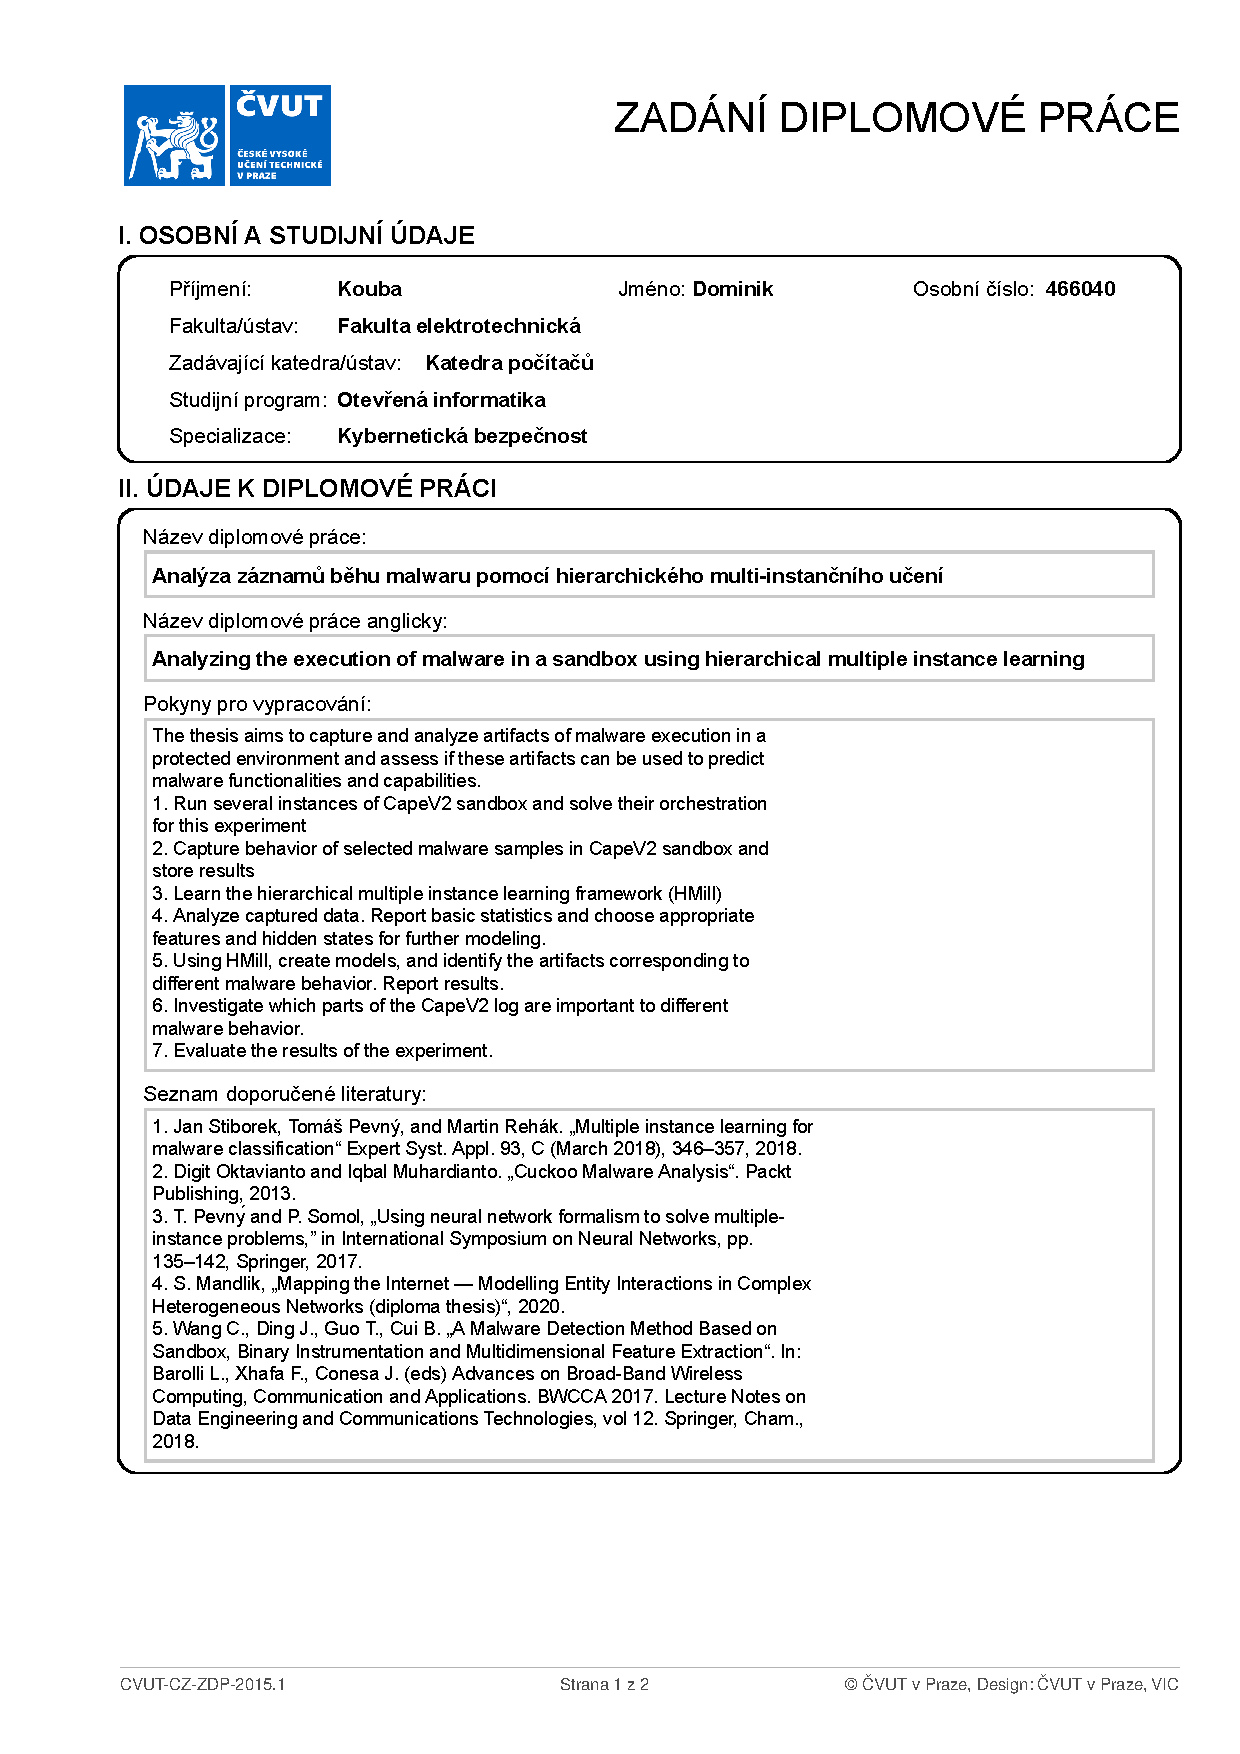
\includepdf[pages=-]{pdfs/zadani.pdf}
		\newpage
	}

	% Title page 
	\coverpagestarts

	% Acknowledgements 
	\acknowledgements
	\noindent
	Zde můžete napsat své poděkování, pokud chcete a máte komu děkovat.

	% Declaration 
	\declaration{In Prague on May 15, 2021}

 	%Abstract 
	\abstractpage

	Translation of Czech abstract into English.

	\vglue60mm

	\noindent{\Huge \textbf{Abstrakt}}
	\vskip 2.75\baselineskip

	\noindent
	Abstrakt práce by měl velmi stručně vystihovat její obsah. Tedy čím se práce zabývá a co je jejím výsledkem/přínosem.

	\noindent
	Očekávají se cca 1 -- 2 odstavce, maximálně půl stránky.

	%%%%%%%%%%%%%%%%%%%%%%%%%%    
	% obsahy a seznamy
	\tableofcontents		% Obsah / Table of Contents 

	% pokud v práci nejsou obrázky nebo tabulky - odstraňte jejich seznam
	\listoffigures			% Obsah / Table of Contents 
	\listoftables			% Seznam tabulek / List of Tables

	%%%%%%%%%%%%%%%%%%%%%%%%%% 
	% TEXT
	\mainbodystarts

	%Chapters
	\chapter{Introduction} \label{chap:intro}
\section*{Motivation}
Nowadays, we face an intense explosion of machine learning applications in various branches of human efforts. We can see applications in biology, chemistry, physics, and others. These technologies are influencing our daily life. They make it easier, faster and more enjoyable. On the other hand, we can see cases where algorithms (especially in machine learning) can control ourselves, our decisions, reasoning, and life.

If we use these computer science tools in a good way, we are often able to create something that may serve our protection. As an example, we can see the detection of threats and frauds in cybersecurity. Research and applications in this particular field are fascinating for multiple reasons, and one of them is motivation. We have to know which side we are standing on and what are the interests of our client.  In the case of fraud detection, we know that the investment is profitable only if the fraud has a significant financial impact. Not all frauds are interesting from the financial point of view because solving them also costs a lot of money. However, from an ethical point of view, every fraud should be punished. 

Similarly, network security, single device security and access control are considered to be applied later or never. Small businesses which are aiming at a specific market are not interested in some stuff which costs much money, and its main impact is preventive. The main role plays financial profit and costs reduction. Nevertheless, nobody wants privacy or data loss. It is often impossible to achieve both. We have to start with an analysis of costs, benefits, risks, their probability and impact (potential damage). This is not so evident in a technical branch as cybersecurity is.

The inseparable character of this play is malware. Let us motivate this thesis by listing several examples.

Firstly, one of the most prevalent malicious software is \emph{ransomware}. Its overall damage is estimated to be $\$20$ billion, and it increases every year \cite{purplesec2021}. The social impact is even more significant than the amount of money. We can see even attacks aiming at healthcare organizations. The first death reported following a ransomware attack was reported in 2020 \cite{Cimpanu2020}.

In Sonic Wall's 2019 report, we can find that IoT malware is becoming more common. It is caused by insufficient protection of these small devices, where we cannot provide complete malware protection. However, $127$ new IoT devices are connected to the internet every second. This leads us to estimate that by the end of 2021 we have 35 billion IoT devices connected to the internet \cite{TheIoTRu52:online}. This risk can not be mitigated easily, and malware elimination will play a significant role as it did so far.

Another convenient trend for malware is widespread encryption which becomes a standard in web traffic. Its main goal is the security of information. However, the creators of malware have much to hide and secure against the protectors, too. The encryption might inform us that the source has something that nobody else should see. A long-lasting trend of such behaviour might be suspicious. We can check if there is a justified reason, or we can at least make some conclusions. But not in a world where everything is encrypted.

$94$~\% of malware was delivered by email in 2020 \cite{Topcyber13:online}. The importance of phishing emails with malicious attachment and other social engineering techniques grows. It is cheaper to produce one sophisticated, convincing email to retrieve some information than attempt to attack a highly protected network perimeter. It also might be used to distribute malware or other threats.

In 2020 AV-atlas \cite{AVATLASM39:online} recorded over 750 million malware samples. At the end of April 2021, it was already 820 million malware samples. The majority of them are executable files attacking windows devices.

Malware research continues, and it undoubtedly will unless we can introduce a solution that is sufficiently universal and flexible to be able to detect zero-day threats (unseen). We might find a solution among machine learning models, which are often involved. However, its challenge is interpretability and explainability, not only in cybersecurity. We face the problem that the performance of the model is often significant, but we are not sure why. It is risky to deploy such a model to a situation where it can meet unseen data. High-quality security engineers do not have to be high-quality machine learning engineers. If we want to involve machine learning methods more and more, we need to be able to interpret and explain its predictions. Then we can combine knowledge from cybersecurity with the results of models and gain a better understanding. 


\section*{Goal}
The main objective of this thesis is to design a pipeline that has a malware file dataset as input and a machine learning model and its explanation as output. We want to go through the whole process, document each step and report results. Our acquisition is the process itself, it is described in detail for the reader to be able to identify problems we experienced and to be able to replicate or extend our setup.

From the assignment of this thesis, we can extract the following steps:
\begin{enumerate}
    \itemsep0em 
    \item Run several instances of CapeV2 \cite{Cape} sandbox and solve their orchestration for this experiment
    \item Capture behaviour of selected malware samples and store results
    \item Learn the hierarchical multiple instance learning framework
    \item Analyze captured data. Report basic statistics and choose appropriate features and hidden states for further modelling
    \item Using HMill, create models and identify the artefacts corresponding to different malware behaviour, report results
    \item Investigate which parts of the CapeV2 log are important to different malware behaviour
\end{enumerate}

The first step implies that we will use dynamic malware analysis to retrieve input for our machine learning model. This is motivated by a couple of thousands of sandbox \emph{JSON} reports we downloaded from the internet and examined. This dataset was not sufficient to observe significant performance. However, it was sufficient to realize that this use case is interesting for further research.

The initial task is data collection. We are about to use \url{https://bazaar.abuse.ch/} as a public data source of malware samples. We chose it because of its free access with no claims in usage and a reasonable amount of samples. We aim at \emph{Portable Executable} (PE), which does not require any additional software running on the target machine. The sandbox we want to use is \emph{CAPEv2} \cite{Cape} because first reports were also produced by this tool, and they are sufficient for analysis purposes.  It is a fork of popular \emph{Cuckoo} sandbox which is no longer maintained. We need to deal with distributed run of the sandbox to be able to collect a sufficient number of samples.

The model we want to use is \emph{hierarchical multiple instance learning} model. In \cite{Mandlik2020} authors showed that this model has significant performance modelling \emph{JSON} documents. We describe it and its alternatives in the first part of the thesis. 

After further research, we decided to model the dependence of malware \emph{signatures} on behavioural features, both presented in \emph{JSON} report. Signatures are the essential input for the original classification techniques used by the sandbox, and we want to see how well the model predicts them based on malware behaviour. We can study the implementation of signatures and their true cause, it might help us with results evaluation.

Finally, we will attempt to explain predictions by choosing a minimal subset of features that contributes to the model predictions the most. The explanation will be performed using the existing \emph{HMill} explainer. Its results will be compared to the original cause of signatures.

\section*{Thesis structure}
The thesis is divided into two main parts. In the first part, we focus on the theoretical background of our method. In the second part, we present a specific setup, our results and their discussion. At the beginning of each chapter is mentioned its particular goal. More complex structures (images, tables) are part of appendices. The thesis also has some attachments, including code, results and examples. These are described in \ref{app:attach}.

The theoretical part starts with the malware analysis theory in chapter \ref{chap:analysis} where we break down the malware itself, types of its analyses and its output. We continue in chapter \ref{chap:classification} where we describe machine learning formalism, cybersecurity context and structured data (\emph{JSON} document) usage in machine learning. Finally, chapters \ref{chap:hmill} and \ref{chap:expth} describe particular methods used in our modelling and explaining experiments.

The second part consists of two chapters. Chapter \ref{chap:infrastructure} includes description of used infrastructure and data collection process. Chapter \ref{chap:results} presents model and explainer setup, results and their discussion.




% The second part breaks down the use case we have. The first chapter \ref{chap:infrastructure} describes malware analysis sample collection, infrastructure and tools used to do that. Following two chapters contain description of the data and reasoning on how to use it and description of training process - hyperparameters, different models, conditions. Finally, last chapter is \ref{chap:expex} where we summarize the model explanation and its results. Crux of the thesis is the dicussion in the chapters \ref{chap:models} and \ref{chap:expex}where we address the model performance and explanation achievements and problems. We follow this discussion in the conlusion and in the formulation of goals of future work.


% The subject of this thesis is malware classification which is part of threat/intrusion detection. We want to use specific machine learning tool - \emph{hierarchical multiple instance learning} to train classifier on the data which we collect ourselves using dynamic malware analysis (\emph{sandboxing}). Our goal is to use data in \emph{JSON} format because this format is quite common output of reporting modules of sandboxes and usualy include majority of the information in structured form. The other reason is that the framework we are about to use shows significant results using such data.

% After we train the classifier (or several) we measure its performance and explain its predicitons. By explanation of predicition we mean using statistical method to extract the most important parts of input vector which contributed the most compared to other parts. Finally we discuss the performance of classifiers and the output of explanation.

% The model could be used to detect malicious code execution based on its behavior and later the explanation can be used to generalize some of our deterministic ways to detect malware (family assignment, signature marking) or just to explain what is for some specific malware family some generic group of malicious programs.

% There are experiments in each part of our task but we would like to examine the whole pipeline to see if we are able to go from plain malware sample to predictor which is explainable. We do not aspire to dig deep in some specific part rather we want to connect each step and identify problems which are in the whole process. We want to see it from a greater prespective. The whole process itself is acquisition and we want to demostrate all the steps.
% \todo{We can add some references}
% \section{Goals}




%%---------------------------------------------------------
% The structure of this thesis follows the steps which we defined in assignement but we solve theoretical point of view and our use case into two parts of this thesis.
% Text is organized such that each chapter focuses on specific goal from the assignement. Firstly we describe theory and prior work, further our conditions, experiments and conclusions.

% The main goal of this thesis which we are aiming at is to capture and analyze artifacts of dynamic malware analyses and draw conclusions in each part of the process. 

% - motivation
% - Motivation behind the modelling itself (classifying itself)
%   - classifying accordig to dynamic analyses, prior arts....
%   - My thesis is more practical, so the main goal is not to compare my results to another ones, but just demonstrate acuuracy of such classifier and everything around like for instance sandboxing, exaplaining
% - goals
% - structure of the thesis

	%\chapter{Úvod}
Výsledná struktura vaší práce a názvy a rozsahy jednotlivých kapitol se samozřejmě budou lišit podle typu práce a podle konkrétní povahy zpracovávaného tématu. 

\section{Jak používat tuto šablonu}

\chapter{Pokyny a návody k formátování textu práce}
Používat se dají všechny příkazy systému \LaTeX. Existuje velké množství volně přístupné dokumentace, tutoriálů, příruček a dalších materiálů v elektronické podobě. Výchozím bodem, kromě Googlu, může být stránka CSTUG (Czech Tech Users Group). Tam najdete odkazy na další materiály.  Vetšinou dostačující a přehledně organizovanou elektronikou dokumentaci najdete například na nebo.

Existují i různé nadstavby nad systémy \TeX{} a \LaTeX, které výrazně usnadní psaní textu zejména začátečníkům. Z mnoha možných uvádíme: Kile\footnote{\url{http://kile.sourceforge.net/}}, TexMaker\footnote{\url{http://www.xm1math.net/texmaker/}}, LyX\footnote{\url{http://www.lyx.org/}}.


\section{Tabulky}
Existuje více způsobů, jak sázet tabulky. Například je možno použít prostředí \verb|table|, které je velmi podobné prostředí \verb|figure|. 

\begin{table}
\begin{center}
\begin{tabular}{|c|l|l|}
\hline
\textbf{DTD} & \textbf{construction} & \textbf{elimination} \\
\hline
$\mid$ & \verb+in1|A|B a:sum A B+ & \verb+case([_:A]a)([_:B]a)ab:A+\\
&\verb+in1|A|B b:sum A B+ & \verb+case([_:A]b)([_:B]b)ba:B+\\
\hline
$+$&\verb+do_reg:A -> reg A+&\verb+undo_reg:reg A -> A+\\
\hline
$*,?$& the same like $\mid$ and $+$ & the same like $\mid$ and $+$\\
& with \verb+emtpy_el:empty+ & with \verb+emtpy_el:empty+\\
\hline
R(a,b) & \verb+make_R:A->B->R+ & \verb+a: R -> A+\\
 & & \verb+b: R -> B+\\
\hline
\end{tabular}
\end{center}
\caption{Ukázka tabulky}
\label{tab:tab1}
\end{table}

Zdrojový text tabulky \ref{tab:tab1} vypadá takto:
\begin{verbatim}
\begin{table}
\begin{center}
\begin{tabular}{|c|l|l|}
\hline
\textbf{DTD} & \textbf{construction} & \textbf{elimination} \\
\hline
$\mid$ & \verb+in1|A|B a:sum A B+ & \verb+case([_:A]a)([_:B]a)ab:A+\\
&\verb+in1|A|B b:sum A B+ & \verb+case([_:A]b)([_:B]b)ba:B+\\
\hline
$+$&\verb+do_reg:A -> reg A+&\verb+undo_reg:reg A -> A+\\
\hline
$*,?$& the same like $\mid$ and $+$ & the same like $\mid$ and $+$\\
& with \verb+emtpy_el:empty+ & with \verb+emtpy_el:empty+\\
\hline
R(a,b) & \verb+make_R:A->B->R+ & \verb+a: R -> A+\\
 & & \verb+b: R -> B+\\
\hline
\end{tabular}
\end{center}
\caption{Ukázka tabulky}
\label{tab:tab1}
\end{table}
\begin{table}
\end{verbatim}

A pokud máte svá data v CSV můžete použít některou z knihoven nabízených v   http://texblog.org/2012/05/30/generate-latex-tables-from-csv-files-excel/ 

\section{Odkazy v textu}
\subsection{Odkazy na literaturu}
Jsou realizovány příkazem \verb|\cite{odkaz}|. 

Seznam literatury je dobré zapsat do samostatného souboru a ten pak zpracovat programem bibtex (viz soubor \verb|reference.bib|). Zdrojový soubor pro \verb|bibtex| vypadá například takto:
\begin{verbatim}
@Article{Chen01,
  author  = "Yong-Sheng Chen and Yi-Ping Hung and Chiou-Shann Fuh",
  title   = "Fast Block Matching Algorithm Based on 
             the Winner-Update Strategy",
  journal = "IEEE Transactions On Image Processing",
  pages   = "1212--1222",
  volume  =  10,
  number  =   8,
  year    = 2001,
}

@Misc{latexdocweb,
  author  = "",
  title   = "{\LaTeX} --- online manuál",
  note    = "\verb|http://www.cstug.cz/latex/lm/frames.html|",
  year    = "",
}
...
\end{verbatim}

%11.12.2008, 3.5.2009
\textbf{Pozor:} Sazba názvů odkazů je dána Bib\TeX{} stylem\\ (\verb|\bibliographystyle{abbrv}|). 
%Budete-li používat české prostředí (\verb|\usepackage[czech]{babel}|), 
Bib\TeX{} tedy obvykle vysází velké pouze počáteční písmeno z názvu zdroje, 
ostatní písmena zůstanou malá bez ohledu na to, jak je napíšete. 
Přesněji řečeno, styl může zvolit pro každý typ publikace jiné konverze. 
Pro časopisecké články třeba výše uvedené, jiné pro monografie (u nich často bývá 
naopak velikost písmen zachována).

Pokud chcete Bib\TeX u napovědět, která písmena nechat bez konverzí 
(viz \texttt{title = "\{$\backslash$LaTeX\} -{}-{}- online manuál"} 
v~předchozím příkladu), je nutné příslušné písmeno (zde celé makro) uzavřít 
do složených závorek. Pro přehlednost je proto vhodné celé parametry 
uzavírat do uvozovek (\texttt{author = "\dots"}), nikoliv do složených závorek.

Odkazy na literaturu ve zdrojovém textu se pak zapisují:
% \begin{verbatim}
% % Podívejte se na %\cite{Chen01}, 
% % další detaily najdete na %\cite{latexdocweb}
% \end{verbatim}

Vazbu mezi soubory \verb|*.tex| a \verb|*.bib| zajistíte příkazem 
\verb|\bibliography{}| v souboru \verb|*.tex|.  V našem případě tedy zdrojový 
dokument \verb|thesis.tex| obsahuje příkaz\\
\verb|\bibliography{reference}|.

Zpracování zdrojového textu s odkazy se provede postupným voláním programů\\
\verb|pdflatex <soubor>| (případně \verb|latex <soubor>|), \verb|bibtex <soubor>| 
a opět\\ \verb|pdflatex <soubor>|.\footnote{První volání \texttt{pdflatex} 
vytvoří soubor s~koncovkou \texttt{*.aux}, který je vstupem pro program 
\texttt{bibtex}, pak je potřeba znovu zavolat program \texttt{pdflatex} 
(\texttt{latex}), který tentokrát zpracuje soubory s příponami \texttt{.aux} a 
\texttt{.tex}. 
Informaci o případných nevyřešených odkazech (cross-reference) vidíte přímo při 
zpracovávání zdrojového souboru příkazem \texttt{pdflatex}. Program \texttt{pdflatex} 
(\texttt{latex}) lze volat vícekrát, pokud stále vidíte nevyřešené závislosti.}


Níže uvedený příklad je převzat z dříve existujících pokynů studentům, kteří 
dělají svou diplomovou nebo bakalářskou práci v~Grafické skupině.\footnote{Několikrát 
jsem byl upozorněn, že web s těmito pokyny byl zrušen, proto jej zde přímo necituji. 
Nicméně příklad sám o sobě dokumentuje obecně přijímaný konsensus ohledně citací 
v~bakalářských a diplomových pracích na KP.} Zde se praví:
\begin{small}
\begin{verbatim}
...
j) Seznam literatury a dalších použitých pramenů, odkazy na WWW stránky, ...
 Pozor na to, že na veškeré uvedené prameny se musíte v textu práce 
 odkazovat -- [1]. 
Pramen, na který neodkazujete, vypadá, že jste ho vlastně nepotřebovali 
a je uveden jen do počtu. Příklad citace knihy [1], článku v časopise [2], 
stati ve sborníku [3] a html odkazu [4]: 
[1] J. Žára, B. Beneš;, and P. Felkel. 
     Moderní počítačová grafika. Computer Press s.r.o, Brno, 1 edition, 1998. 
     (in Czech). 
[2] P. Slavík. Grammars and Rewriting Systems as Models for Graphical User 
     Interfaces. Cognitive Systems, 4(4--3):381--399, 1997. 
[3] M. Haindl, Š. Kment, and P. Slavík. Virtual Information Systems. 
     In WSCG'2000 -- Short communication papers, pages 22--27, Pilsen, 2000. 
     University of West Bohemia. 
[4] Knihovna grafické skupiny katedry počítačů: 
     http://www.cgg.cvut.cz/Bib/library/ 
\end{verbatim}
\end{small}
% \ldots{} abychom výše citované odkazy skutečně našli v (automaticky generovaném) seznamu literatury tohoto textu, musíme je nyní alespoň jednou citovat: Kniha \cite{kniha}, článek v~časopisu \cite{clanek}, příspěvek na konferenci \cite{sbornik}, www odkaz \cite{www}.

% Ještě přidáme další ukázku citací online zdrojů podle české normy. Odkaz na wiki o frameworcich \cite{wiki:framework} a ORM \cite{wiki:orm}. Použití viz soubor \verb|reference.bib|. V seznamu literatury by nyní měly být živé odkazy na zdroje. V \verb|reference.bib| je zcela nový typ publikace. Detaily dohledal a dodal Petr Dlouhý v dubnu 2010. Podrobnosti najdete ve zdrojovém souboru tohoto textu v komentáři u příkazu \verb|\thebibliography|.

\subsection{Odkazy na obrázky, tabulky a kapitoly}
\begin{itemize}
\item Označení místa v textu, na které chcete později čtenáře práce odkázat, se provede příkazem \verb|\label{navesti}|. Lze použít v prostředích \verb|figure| a  \verb|table|, ale též za názvem kapitoly nebo podkapitoly.
\item Na návěští se odkážeme příkazem \verb|\ref{navesti}| nebo \verb|\pageref{navesti}|.
\end{itemize}

\section{Rovnice, centrovaná, číslovaná matematika}
Jednoduchý matematický výraz zapsaný přímo do textu se vysází pomocí prostředí \verb|math|, resp. zkrácený zápis pomocí uzavření textu rovnice mezi znaky \verb|$|.

Kód \verb|$ S = \pi * r^2 $| bude vysázen takto: $ S = \pi * r^2 $.

Pokud chcete nečíslované rovnice, ale umístěné centrovaně na samostatné řádky, pak lze použít prostředí \verb|displaymath|, resp. zkrácený zápis pomocí uzavření textu rovnice mezi znaky \verb|$$|. Zdrojový kód: 
\begin{verb}
|$$ S = \pi * r^2 $$|
\end{verb}
bude pak vysázen takto:
$$ S = \pi * r^2 $$

Chcete-li mít rovnice číslované, je třeba použít prostředí \verb|eqation|. Kód:
\begin{verbatim}
\begin{equation}
  S = \pi * r^2
\end{equation}

\begin{equation}
  V = \pi * r^3
\end{equation}
\end{verbatim}
je potom vysázen takto:
\begin{equation}
  S = \pi * r^2
\end{equation}

\begin{equation}
  V = \pi * r^3
\end{equation}

\section{Kódy a algoritmy}
\subsection{Zdrojové kódy}
Chceme-li vysázet například část zdrojového kódu programu, hodí se prostředí \verb|verbatim|, které je bez formátování: 
\begin{verbatim}
         (* nickname2 *)
Lego> Refine in1
             (do_reg (nickname1 h));
Refine by  in1 (do_reg (nickname1 h))
   ?4 : pcdata
   ?5 : pcdata
          (* surname2 *)
Lego> Refine surname1 h;
Refine by  surname1 h
   ?5 : pcdata
          (* email2 *)
Lego> Refine undo_reg (email1 h);
Refine by  undo_reg (email1 h)
*** QED ***
\end{verbatim}

nebo se dá použít \verb|listings|, což je package, který umožňuje i syntax higlighting podle jazyka:

\lstset{language=Python} %následuje python kód a použije se python syntax
\begin{lstlisting}
	print 'Hello, world!'
\end{lstlisting}

a umožňuje načíst i přiložené zdrojové soubory:

\lstinputlisting[language=C]{code/hello.c}

\subsection{Algoritmy}
Pokud chcete v práci popsat obecné algoritmy s využitím pseudokódu, můžete použít knihovny \verb|algorithmicx| a \verb|algpseudocode|:
\begin{algorithmic}
\If {$i\geq maxval$}
    \State $i\gets 0$
\Else
    \If {$i+k\leq maxval$}
        \State $i\gets i+k$
    \EndIf
\EndIf
\end{algorithmic}

\section{Zkratky}
% V tomto textu používám několik zkratek, třeba 2D\nomenclature{2D}{Two-Dimensional} nebo \nomExpl{KNB}{Killing nanobots}. V úvodní části dokumentu můžete nastavit/upravit příkaz pro zadání zkratky, pokud např. chcete mít význam zkratky pod čarou. Všechny zkratky se vytisknou podle abecedy (\nom{ABC}{Zkratka pro abecedu}) v příloze \ref{apx:zkratky}, aby toto fungovalo musíte \cite{Amerini2020} vybudovat index pomocí příkazu:
\begin{verbatim}
		makeindex soubor.nlo -s nomencl.ist -o soubor.nls
\end{verbatim}

\section{České uvozovky}
V souboru \verb|k336_thesis_macros.tex| je příkaz \verb|\uv{}| pro sázení českých uvozovek. \uv{Text uzavřený do českých uvozovek.}

\chapter{Závěr}

\begin{itemize}
\item Zhodnocení splnění cílů DP/BP a  vlastního přínosu práce (při formulaci je třeba vzít v potaz zadání práce).
\item Diskuse dalšího možného pokračování práce.
\end{itemize} 


%%%%%%%%%%%%%%%%%%%%%%%%%% 
% Seznam literatury je v samostatnem souboru reference.bib. Ten
% upravte dle vlastnich potreb, potom zpracujte (a do textu
% zapracujte) pomoci prikazu bibtex a nasledne pdflatex (nebo
% latex). Druhy z nich alespon 2x, aby se poresily odkazy.

% originally following specification for bibliography formating was used
%\bibliographystyle{abbrv}

% Here is an improvment by Petr Dlouhy (April 2010).
% It is mainly for supervisors who expect Czech fomrating rules for references
% Additional feature is live url addresses to sources from your pdf file
% It requires the file csplainnat.bst (included in this sample zipfile).

	%\section{Obrázky}
Obrázky jsou vhodným nástrojem pro ilustraci a doplnění textu, používejte je v rozumné míře ať vaše práce nepřipomíná komix. Při hledání/tvorbě obrázků nezapomeňte na to, že u přejatých obrázků musíte odkazovat jejich zdroj a že obrázky by měly být čitelné (typicky .jpg soubory se často rozostří). Dalším častým neduhem jsou obrázky s anglickými popisky v česky psaném textu, pokud to je možné udržte jazyk práce jednotný.

\subsection{Vkládání obrázků}
Obrázky se umísťují do plovoucího prostředí \verb|figure|. Každý obrázek by měl obsahovat \textbf{název} (\verb|\caption|) a \textbf{návěští} (\verb|\label|). Použití příkazu pro vložení obrázku \\\verb|\includegraphics| je podmíněno aktivací (načtením) balíku graphicx příkazem\\ \verb|\usepackage{graphicx}|.

Budete-li zdrojový text zpracovávat pomocí programu \verb|pdflatex|, očekávají se obrázky s příponou \verb|*.pdf|\footnote{pdflatex umí také formáty PNG a JPG.}, použijete-li k formátování \verb|latex|, očekávají se obrázky s příponou \verb|*.eps|.\footnote{Vzájemnou konverzi mezi snad všemi typy obrazku včetně změn vekostí a dalších vymožeností vám může zajistit balík ImageMagic  (http://www.imagemagick.org/script/index.php). Je dostupný pod Linuxem, Mac OS i MS Windows. Důležité jsou zejména příkazy convert a identify.}

\begin{figure}[ht]
\begin{center}
\includegraphics[width=5cm]{figures/LogoCVUT}
\caption{Popiska obrázku}
\label{fig:logo}
\end{center}
\end{figure}

Příklad vložení obrázku:
\begin{verbatim}
\begin{figure}[h]
\begin{center}
\includegraphics[width=5cm]{figures/LogoCVUT}
\caption{Popiska obrazku}
\label{fig:logo}
\end{center}
\end{figure}
\end{verbatim}

\subsection{Kreslení obrázků}
Zřejmě každý z vás má nějaký oblíbený nástroj pro tvorbu obrázků. Jde jen o to, abyste dokázali obrázek uložit v požadovaném formátu nebo jej do něj konvertovat (viz předchozí kapitola). Je zřejmě vhodné kreslit obrázky vektorově. Celkem oblíbený, na ovládání celkem jednoduchý a přitom dostatečně mocný je například program Inkscape.

Zde stojí za to upozornit na kreslící programe Ipe, který dokáže do obrázku vkládat komentáře přímo v latexovském formátu (vzroce, stejné fonty atd.). Podobné věci umí na Linuxové platformě nástroj Xfig. 

Za pozornost ještě stojí schopnost editoru Ipe importovat obrázek (jpg nebo bitmap) a krelit do něj latexovské popisky a komentáře. Výsledek pak umí exportovat přímo do pdf.

Další možností je knihovna graphviz, které vykreslí obrázek podle vašeho popisu (kódu), výstup je možný do mnoha formátů (.eps, .jpg, ...).



	%Biblio
	\bibliographystyle{alpha}
	%\bibliographystyle{csplainnat}
	%bibliographystyle{plain}
	% \bibliographystyle{psc}
	%\bibliographystyle{apalike}
	{
	\bibliography{bib/Master_thesis}
	}

	%%%%%%%%%%%%%%%%%%%%%%%%%% 
	% APPENDIX
	\appendix	

	\printnomenclature
	\label{apx:zkratky}

	\chapter{Obsah přiloženého CD}
	\textbf{\large Tato příloha je povinná pro každou práci. Každá práce musí totiž obsahovat přiložené CD. Viz dále.}

	% Může vypadat například takto. Váš seznam samozřejmě bude odpovídat typu vaší práce. (viz \cite{infodp}):

	% \begin{figure}[h]
	% \begin{center}
	% \includegraphics[width=14cm]{figures/seznamcd}
	% \caption{Seznam přiloženého CD --- příklad}
	% \label{fig:seznamcd}
	% \end{center}
	% \end{figure}

	% Na GNU/Linuxu si strukturu přiloženého CD můžete snadno vyrobit příkazem:\\ 
	% \verb|$ tree . >tree.txt|\\
	% Ve vzniklém souboru pak stačí pouze doplnit komentáře.

	% Z \textbf{README.TXT} (případne index.html apod.)  musí být rovněž zřejmé, jak programy instalovat, spouštět a jaké požadavky mají tyto programy na hardware.

	% Adresář \textbf{text}  musí obsahovat soubor s vlastním textem práce v PDF nebo PS formátu, který bude později použit pro prezentaci diplomové práce na WWW.

\end{document}
